 \documentclass[11pt]{article}
\usepackage[letterpaper, margin=1in]{geometry} % [letterpaper, margin=1in]
\usepackage[english]{babel}
\usepackage[utf8]{inputenc}
\usepackage{fancyhdr}
\usepackage{booktabs}
\usepackage{amsmath}
\usepackage{textcomp}
\usepackage{gensymb}
\usepackage{graphicx}
\usepackage{floatrow}
\usepackage{hyperref}
\usepackage{lastpage}

\newcommand\blfootnote[1]{%
  \begingroup
  \renewcommand\thefootnote{}\footnote{#1}%
  \addtocounter{footnote}{-1}%
  \endgroup
}

\def \hfillx {\hspace*{-\textwidth} \hfill}

\usepackage{hyperref}

\pagestyle{fancy}
\fancyhf{}
\rhead{Paras Jain // pjain67}
\lhead{CS4641 Project 4: Reinforcement Learning}
\cfoot{\thepage}

\title{CS4641: Reinforcement Learning}
\author{Paras Jain}
\date{}

\begin{document}

\maketitle

\begin{abstract}
This report details an exploration of Reinforcement Learning through \textit{Value Iteration}, \textit{Policy Iteration}, \textit{Q-Learning} and \textit{Prioritized Sweeping}.
\end{abstract}

\section{Reinforcement Learning Background}
...

% Come up with two interesting MDPs. Explain why they are interesting. They don't need to be overly complicated or directly grounded in a real situation, but it will be worthwhile if your MDPs are inspired by some process you are interested in or are familiar with. It's ok to keep it somewhat simple. For the purposes of this assignment, though, make sure one has a "small" number of states, and the other has a "large" number of states.
\section{Markov Decision Processes Chosen}
Two Markov decision processes were chosen of the same family of Gridworld MDPs (as covered in class). Two problems of the same class were chosen from the same class to compare how problem size affects.

The GridWorld MDP is where an agent is on a grid of squares and the goal is to reach some goal state. In order to encourage the agent to converge to a solution, there is a penalty of $-1$ for being in a state. Hitting a wall has a penalty of $-50$.

\begin{figure}[h]
    \begin{floatrow}
        \ffigbox{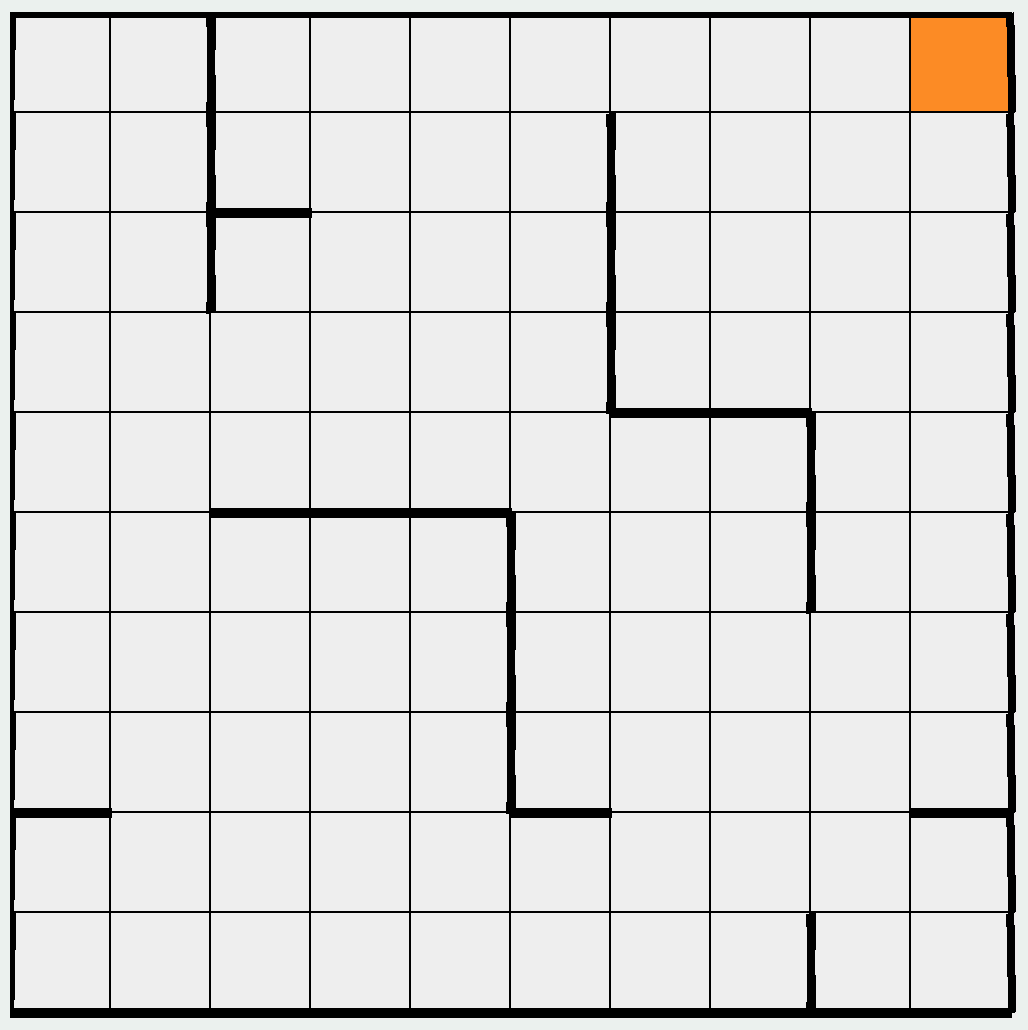
\includegraphics[width=.3\textwidth]{pics/medium}}{\centering\caption{Medium map. Goal state in orange.}\label{fig:mediummap}}
        \ffigbox{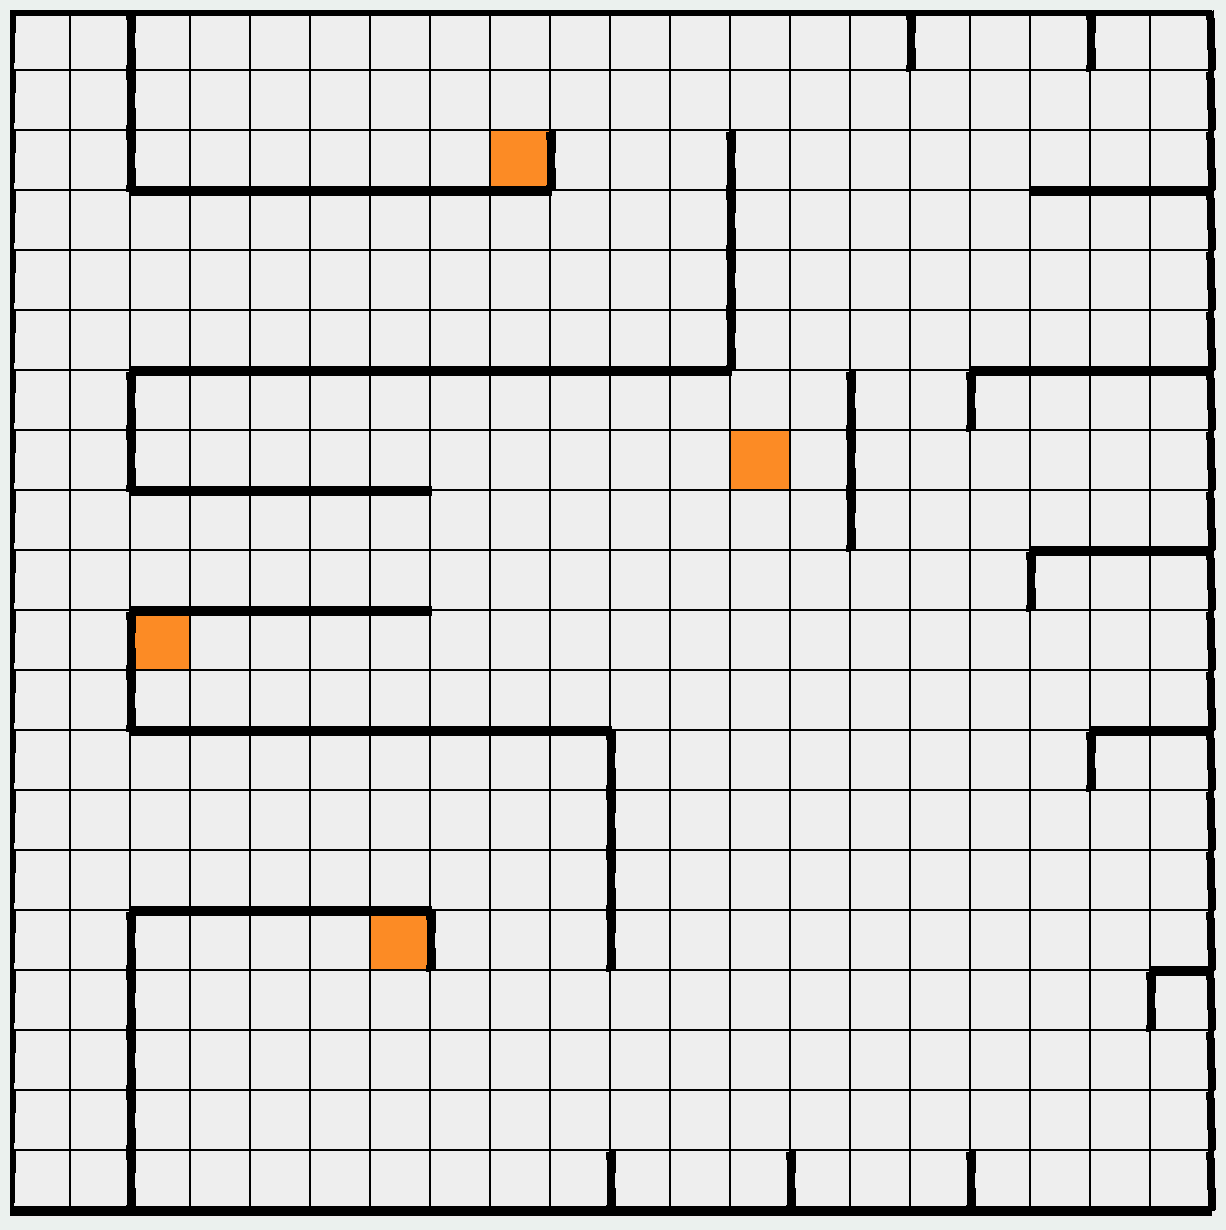
\includegraphics[width=.3\textwidth]{pics/big}}{\centering\caption{Large map. Goal state in orange.}\label{fig:bigmap}}
    \end{floatrow}
\end{figure}

Each state has a transition function Equation \ref{eq:mdptransition}, parametrized by probability $p$ which represents the probability of the transition not going as intended.

\begin{equation}
\label{eq:mdptransition}
S_{n+1}(x) = 
\begin{cases}
    x,& \text{with probability } 1-p\\
    rotate(x, 90\degree),              & \text{with probability } \frac{p}{2}\\
    rotate(x, -90\degree),              & \text{with probability } \frac{p}{2}
\end{cases}
\end{equation}

The medium map was designed to be relatively small with wide spaces with limited numbers of walls - refer to Figure \ref{fig:mediummap}. It is $10 \times 10$ with 100 total states. There is a single goal.

The large map was designed to have avenues with walls of varying configurations (varying length/width/direction avenues) - refer to Figure \ref{fig:bigmap}. It is $20 \time 20$ with 400 total states.

\subsection{MDP Interest}
I chose Gridworld as it is the most common example of reinforcement learning that students learn. The problem has received a huge amount of research attention and are relatively well understood. By choosing two instances of the same MDP class, we can compare the effect that board size has on the results.

For the large map, there are multiple goals in comparison to a single goal with the small map, which will be interesting to compare to the medium map. The placement of the goals is generally near walls which makes the direction of approach to a goal important.

The multiple avenues should reveal some interesting conclusions regarding exploration versus exploitation.



\section{Phase 1 - Value Iteration/Policy Iteration}

For the analysis on value iteration and policy iteration, RLSim\footnote{\url{http://www.cs.cmu.edu/~awm/rlsim/}} was used.

\subsection{Value Iteration}

\begin{table}[h!]
    \begin{minipage}{0.5\textwidth}
        \centering
        \textbf{Medium map}\\
        \begin{tabular}{@{}c|cc@{}}
        \toprule
        \textbf{$p$} & \textbf{Iterations} & \textbf{Time taken (ms)} \\ \midrule
        0.0          & 19                            & 51                       \\
        0.1          & 40                            & 20                       \\
        0.2          & 62                            & 29                       \\
        0.3          & 90                            & 48                       \\
        0.4          & 132                           & 85                       \\
        0.5          & 203                           & 89                       \\
        0.6          & 417                           & 196                      \\
        0.7          & 1821                          & 907                      \\
        0.8          & 2178                          & 1216                     \\
        0.9          & 679                           & 299                      \\
        1.0          & 708                           & 332                      \\ \bottomrule
        \end{tabular}
    \end{minipage}
    \hfillx
    \begin{minipage}{0.5\textwidth}
        \centering
        \textbf{Large map}\\
        \begin{tabular}{@{}c|cc@{}}
        \toprule
        \textbf{$p$} & \textbf{Iterations} & \textbf{Time taken (ms)} \\ \midrule
        0.0          & 18                  & 60                       \\
        0.1          & 37                  & 128                      \\
        0.2          & 54                  & 173                      \\
        0.3          & 80                  & 259                      \\
        0.4          & 127                 & 411                      \\
        0.5          & 193                 & 622                      \\
        0.6          & 420                 & 1397                     \\
        0.7          & 1503                & 5113                     \\
        0.8          & 1760                & 5910                     \\
        0.9          & 678                 & 2224                     \\
        1.0          & 471                 & 1560                     \\ \bottomrule
        \end{tabular}
    \end{minipage}
    \caption{Value iteration results for both maps. Note that $p$ is the probability of state transition error.}\label{table:valueitertable}
\end{table}

\begin{figure}[h!]
    \begin{floatrow}
        \ffigbox{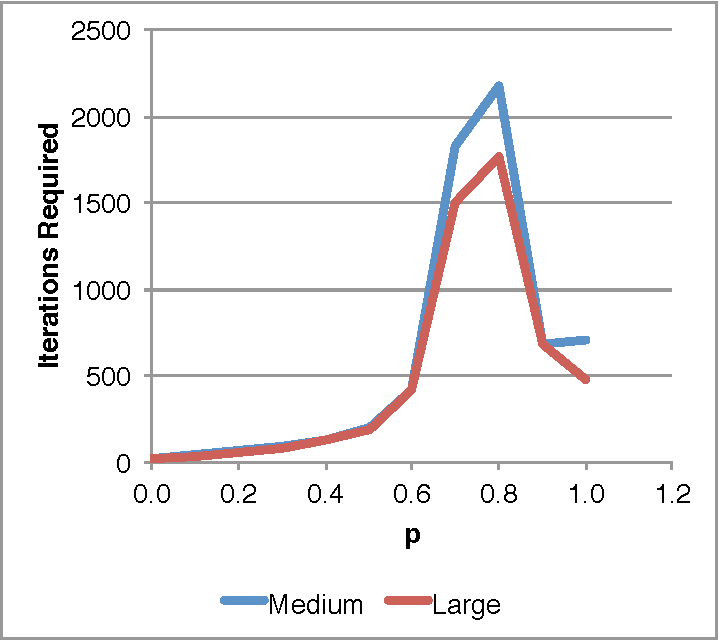
\includegraphics[width=.5\textwidth]{pics/ValueIterationIterations}}{\caption{Iterations to convergence for Value Iteration for both maps.}\label{fig:valueiterationiterations}}
        \ffigbox{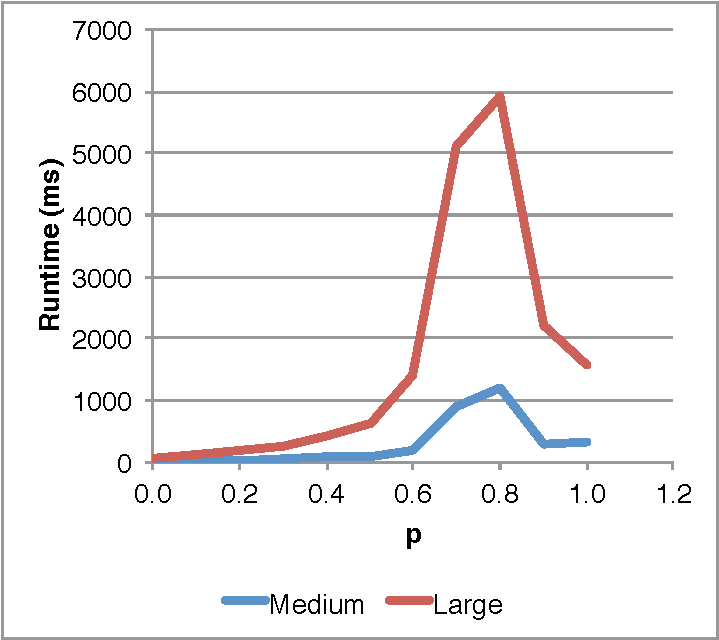
\includegraphics[width=.5\textwidth]{pics/ValueIterationRuntime}}{\caption{Runtime to convergence for Value Iteration for both maps.}\label{fig:valueiterationruntime}}
    \end{floatrow}
\end{figure}

\subsection{Policy Iteration}

\begin{table}[h!]
    \begin{minipage}{0.5\textwidth}
        \centering
        \textbf{Medium map}\\
        \begin{tabular}{@{}c|cc@{}}
        \toprule
        \textbf{$p$} & \textbf{Iterations} & \textbf{Time taken (ms)} \\ \midrule
        0.0          & 13       & 65                     \\
        0.1          & 8       & 52                     \\
        0.2          & 7       & 60                     \\
        0.3          & 5       & 31                     \\
        0.4          & 6       & 48                     \\
        0.5          & 6       & 58                     \\
        0.6          & 5       & 111                     \\
        0.7          & 3       & 99                     \\
        0.8          & 5       & 33                     \\
        0.9          & 6       & 17                     \\
        1.0          & 13       & 13                     \\ \bottomrule
        \end{tabular}
    \end{minipage}
    \hfillx
    \begin{minipage}{0.5\textwidth}
        \centering
        \textbf{Large map}\\
        \begin{tabular}{@{}c|cc@{}}
        \toprule
        \textbf{$p$} & \textbf{Iterations} & \textbf{Time taken (ms)} \\ \midrule
        0.0          & 15       & 624                     \\
        0.1          & 13       & 618                     \\
        0.2          & 18       & 344                     \\
        0.3          & 15       & 414                     \\
        0.4          & 9       & 327                     \\
        0.5          & 8       & 493                     \\
        0.6          & 6       & 898                     \\
        0.7          & 7       & 1273                     \\
        0.8          & 7       & 197                     \\
        0.9          & 30       & 169                     \\
        1.0          & 33       & 131                     \\ \bottomrule
        \end{tabular}
    \end{minipage}
    \caption{Policy iteration results for both maps. Note that $p$ is the probability of state transition error.}\label{table:valueitertable}
\end{table}

\begin{figure}[h!]
    \begin{floatrow}
        \ffigbox{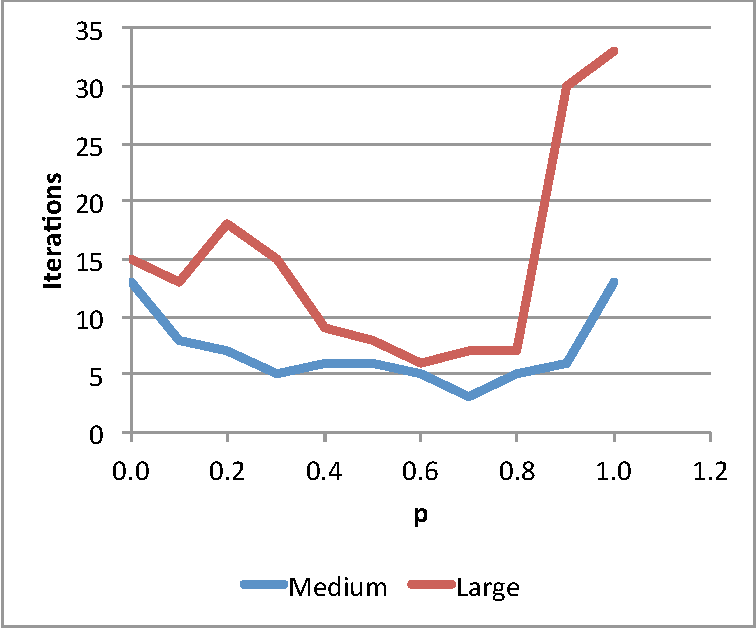
\includegraphics[width=.5\textwidth]{pics/PolicyIterationIterations}}{\caption{Iterations to convergence for Policy Iteration for both maps.}\label{fig:policyiterationiterations}}
        \ffigbox{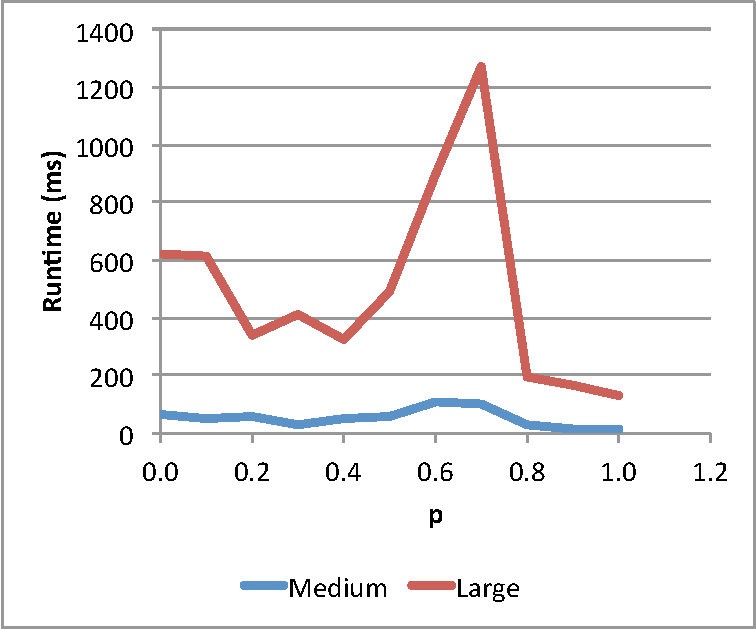
\includegraphics[width=.5\textwidth]{pics/PolicyIterationRuntime}}{\caption{Runtime to convergence for Policy Iteration for both maps.}\label{fig:policyiterationruntime}}
    \end{floatrow}
\end{figure}

\section{Phase 2 - Q-Learning and Prioritized Sweeping}

\subsection{Q-Learning}

To study Q-learning, I modeled the parameter space to analyze the two key performance metrics of a RL algorithm - runtime and utility achieved. Iterations was fixed in this case in order to be able to visualize the highly-dimensional parameter space to produce meaningful conclusions.

Refer to Figure \ref{fig:qlscatter}\footnote{For an interactive 3D scatter plot, see \url{https://plot.ly/~parasj/4.embed}} and Figure \ref{fig:qlscatterbig}\footnote{For an interactive 3D scatter plot, see \url{https://plot.ly/~parasj/6.embed}} for visualization of the parameter space over $p$, $\epsilon$ and scores.

\begin{figure}[h]
    \begin{floatrow}
        \ffigbox{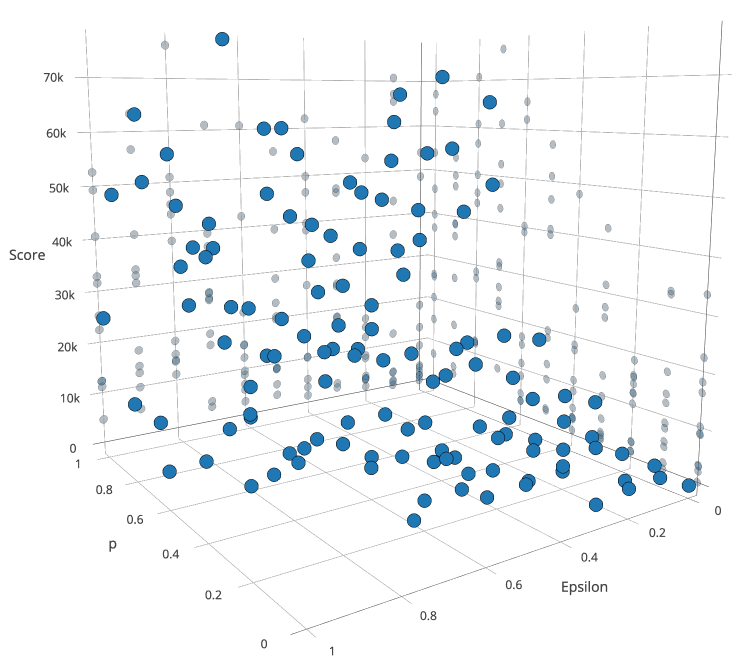
\includegraphics[width=.5\textwidth]{pics/medium03_scatter}}{\centering\caption{Q-Learning scores for the medium map over a space of $p$ and $\epsilon$ values, visualized as a 3D scatter plot.}\label{fig:qlscatter}}
        \ffigbox{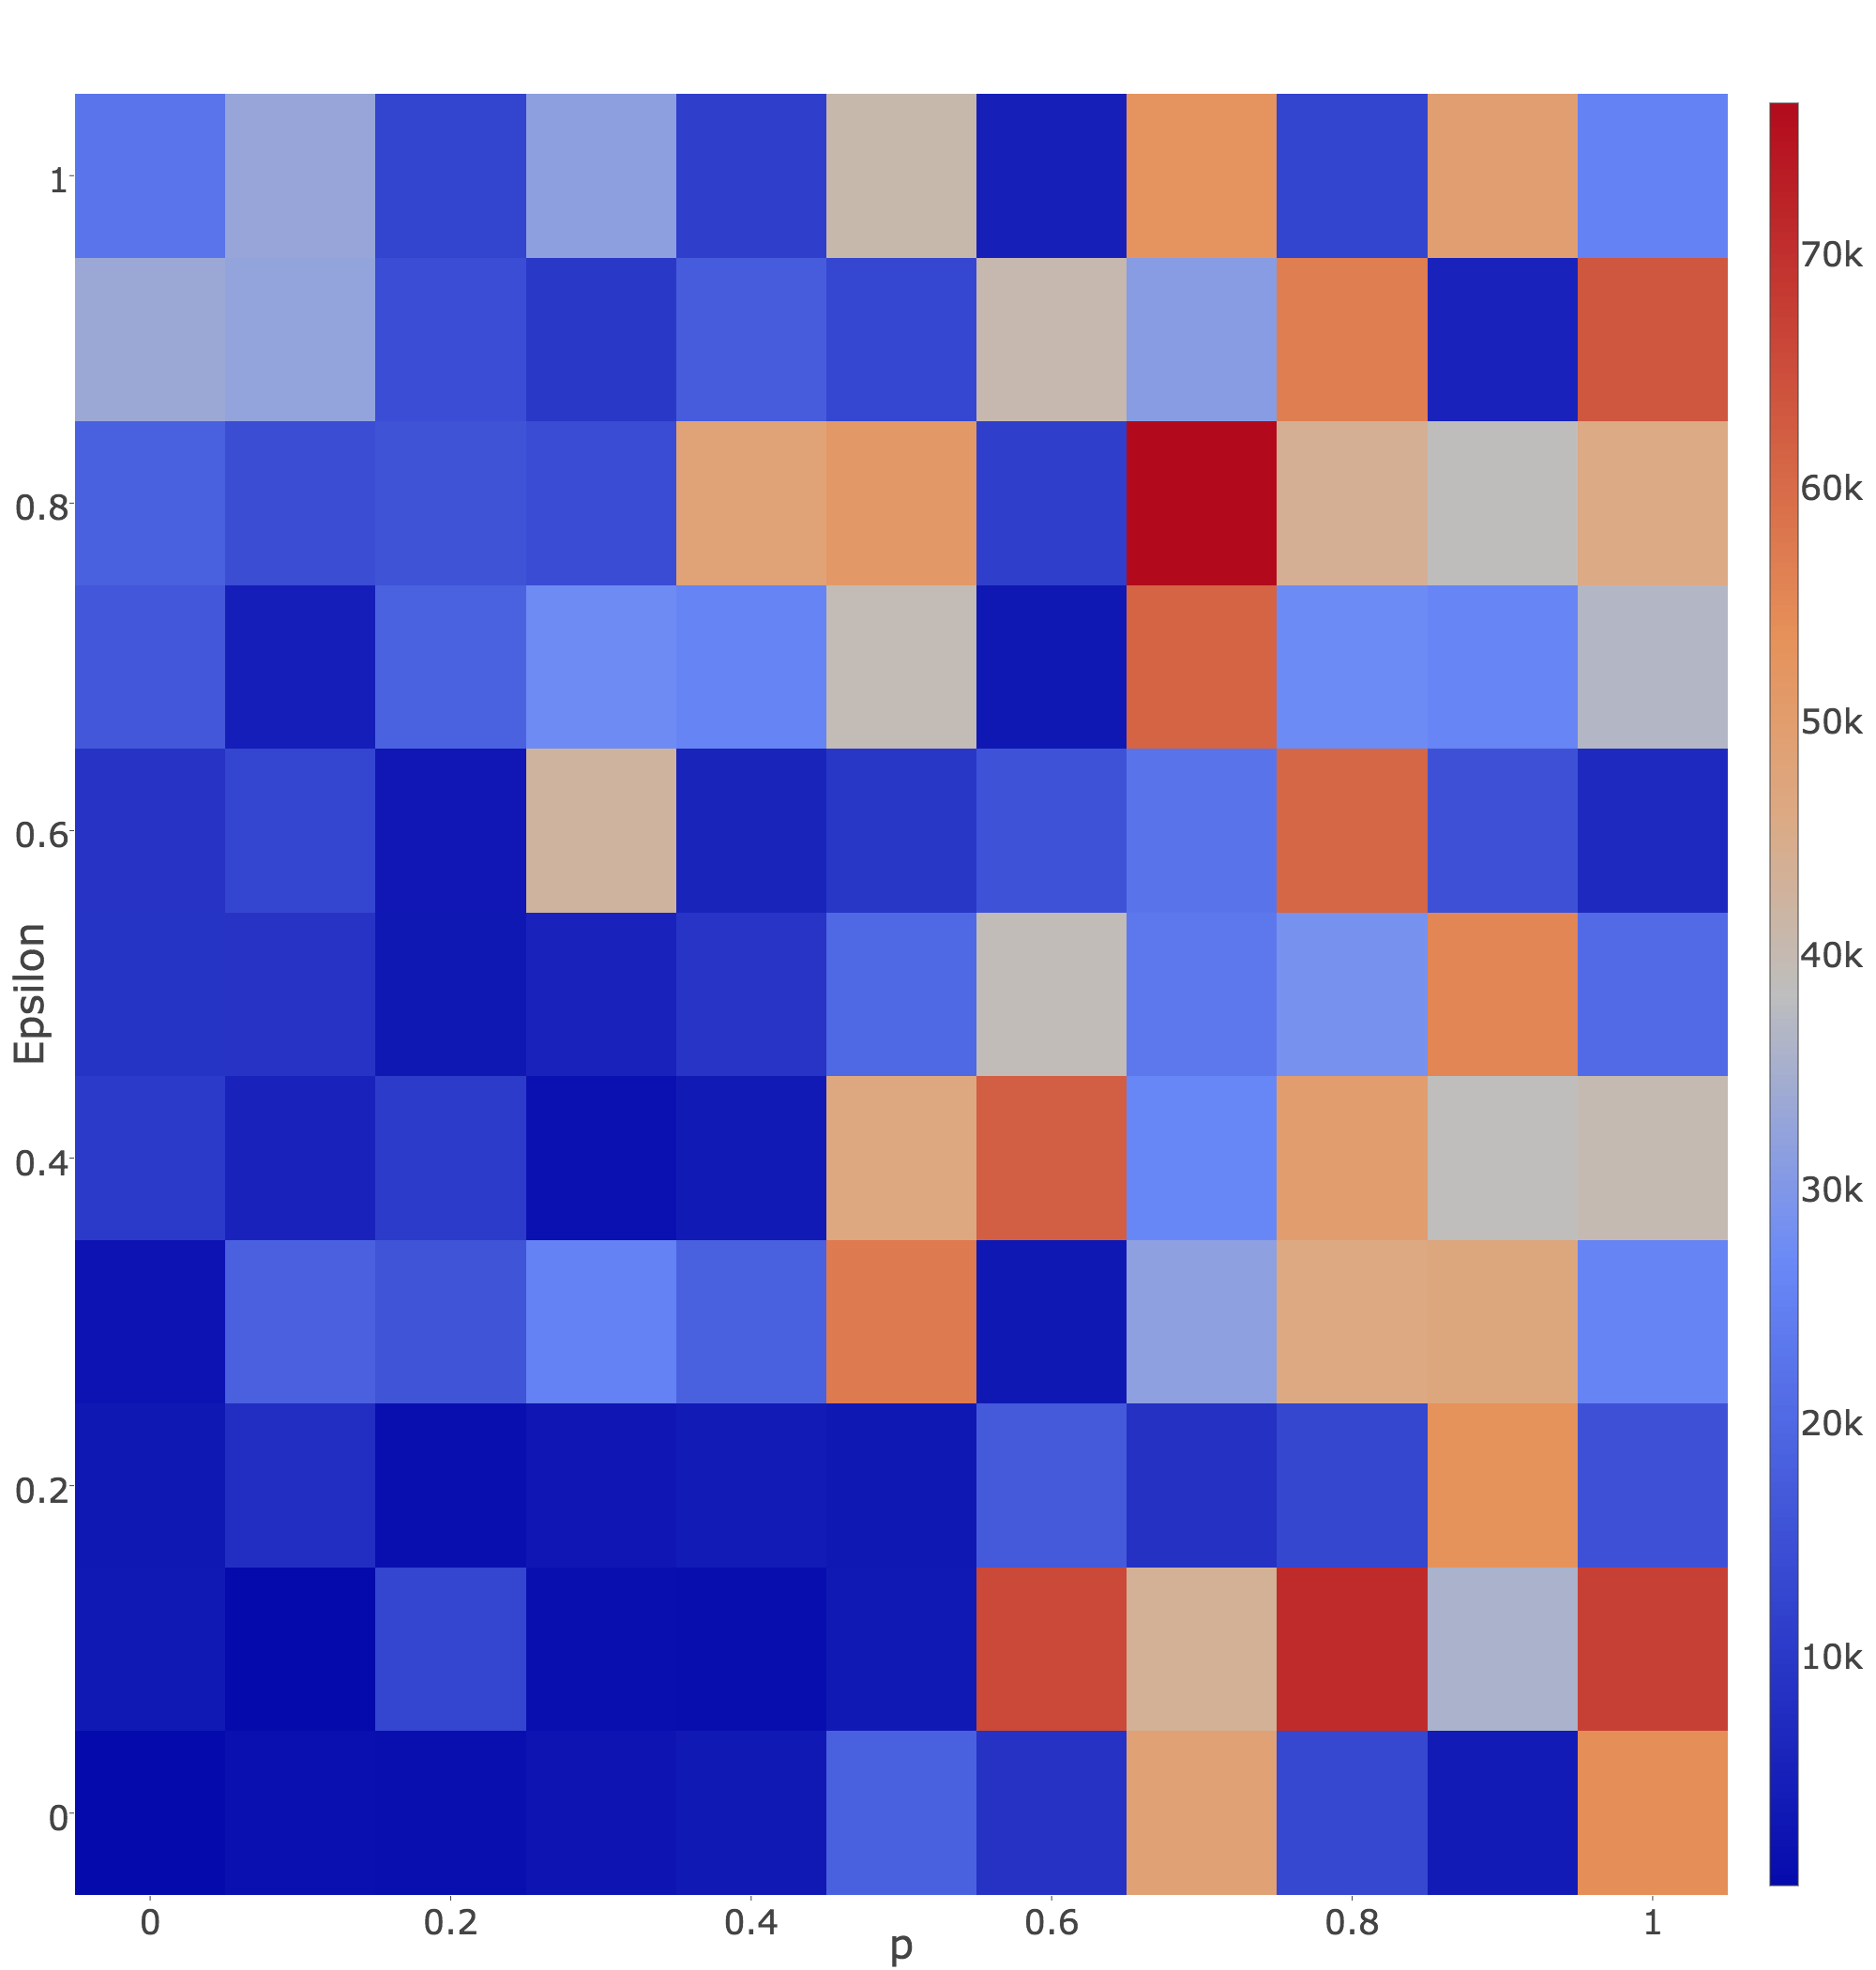
\includegraphics[width=.5\textwidth]{pics/medium03_heatmap}}{\centering\caption{Q-Learning scores for the medium map over a space of $p$ and $\epsilon$ values, visualized as a heatmap.}\label{fig:qlheatmap}}
    \end{floatrow}
\end{figure}

\begin{figure}[h]
    \begin{floatrow}
        \ffigbox{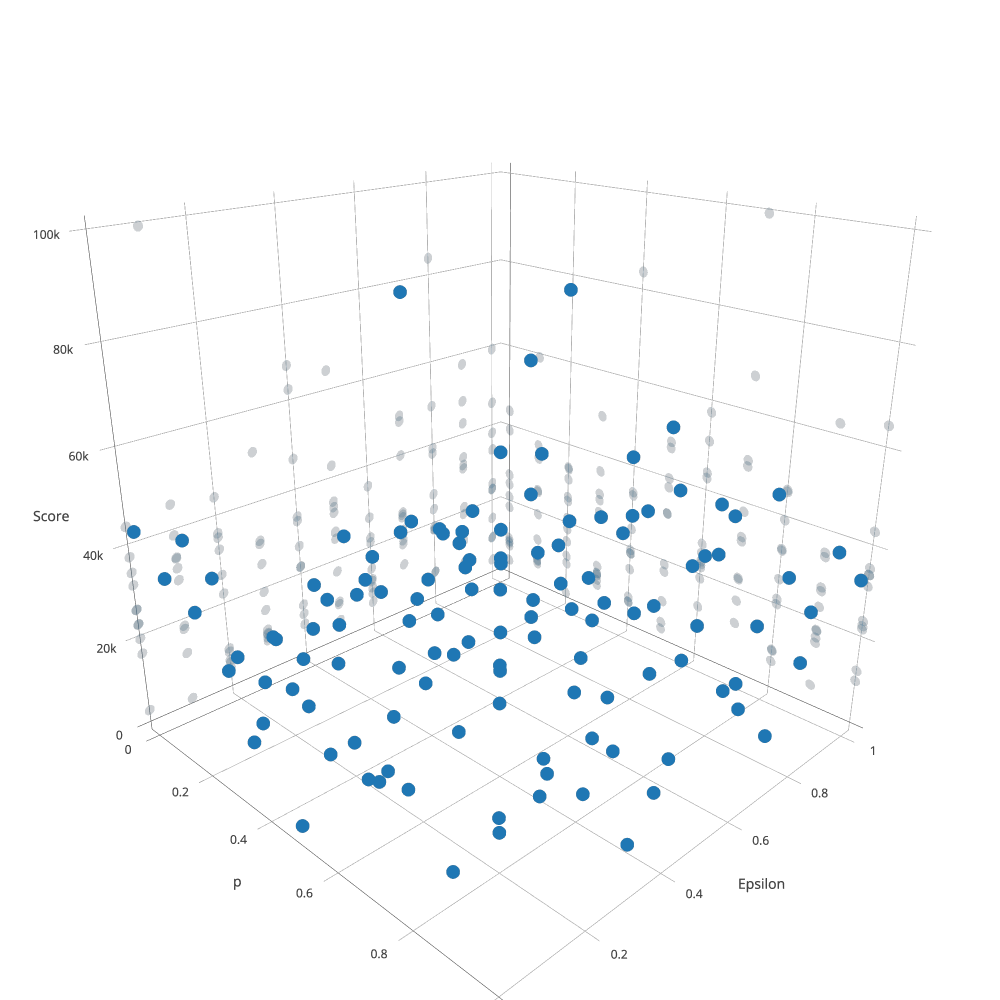
\includegraphics[width=.5\textwidth]{pics/QLearningBig}}{\centering\caption{Q-Learning scores for the big map over a space of $p$ and $\epsilon$ values, visualized as a 3D scatter plot.}\label{fig:qlscatterbig}}
        \ffigbox{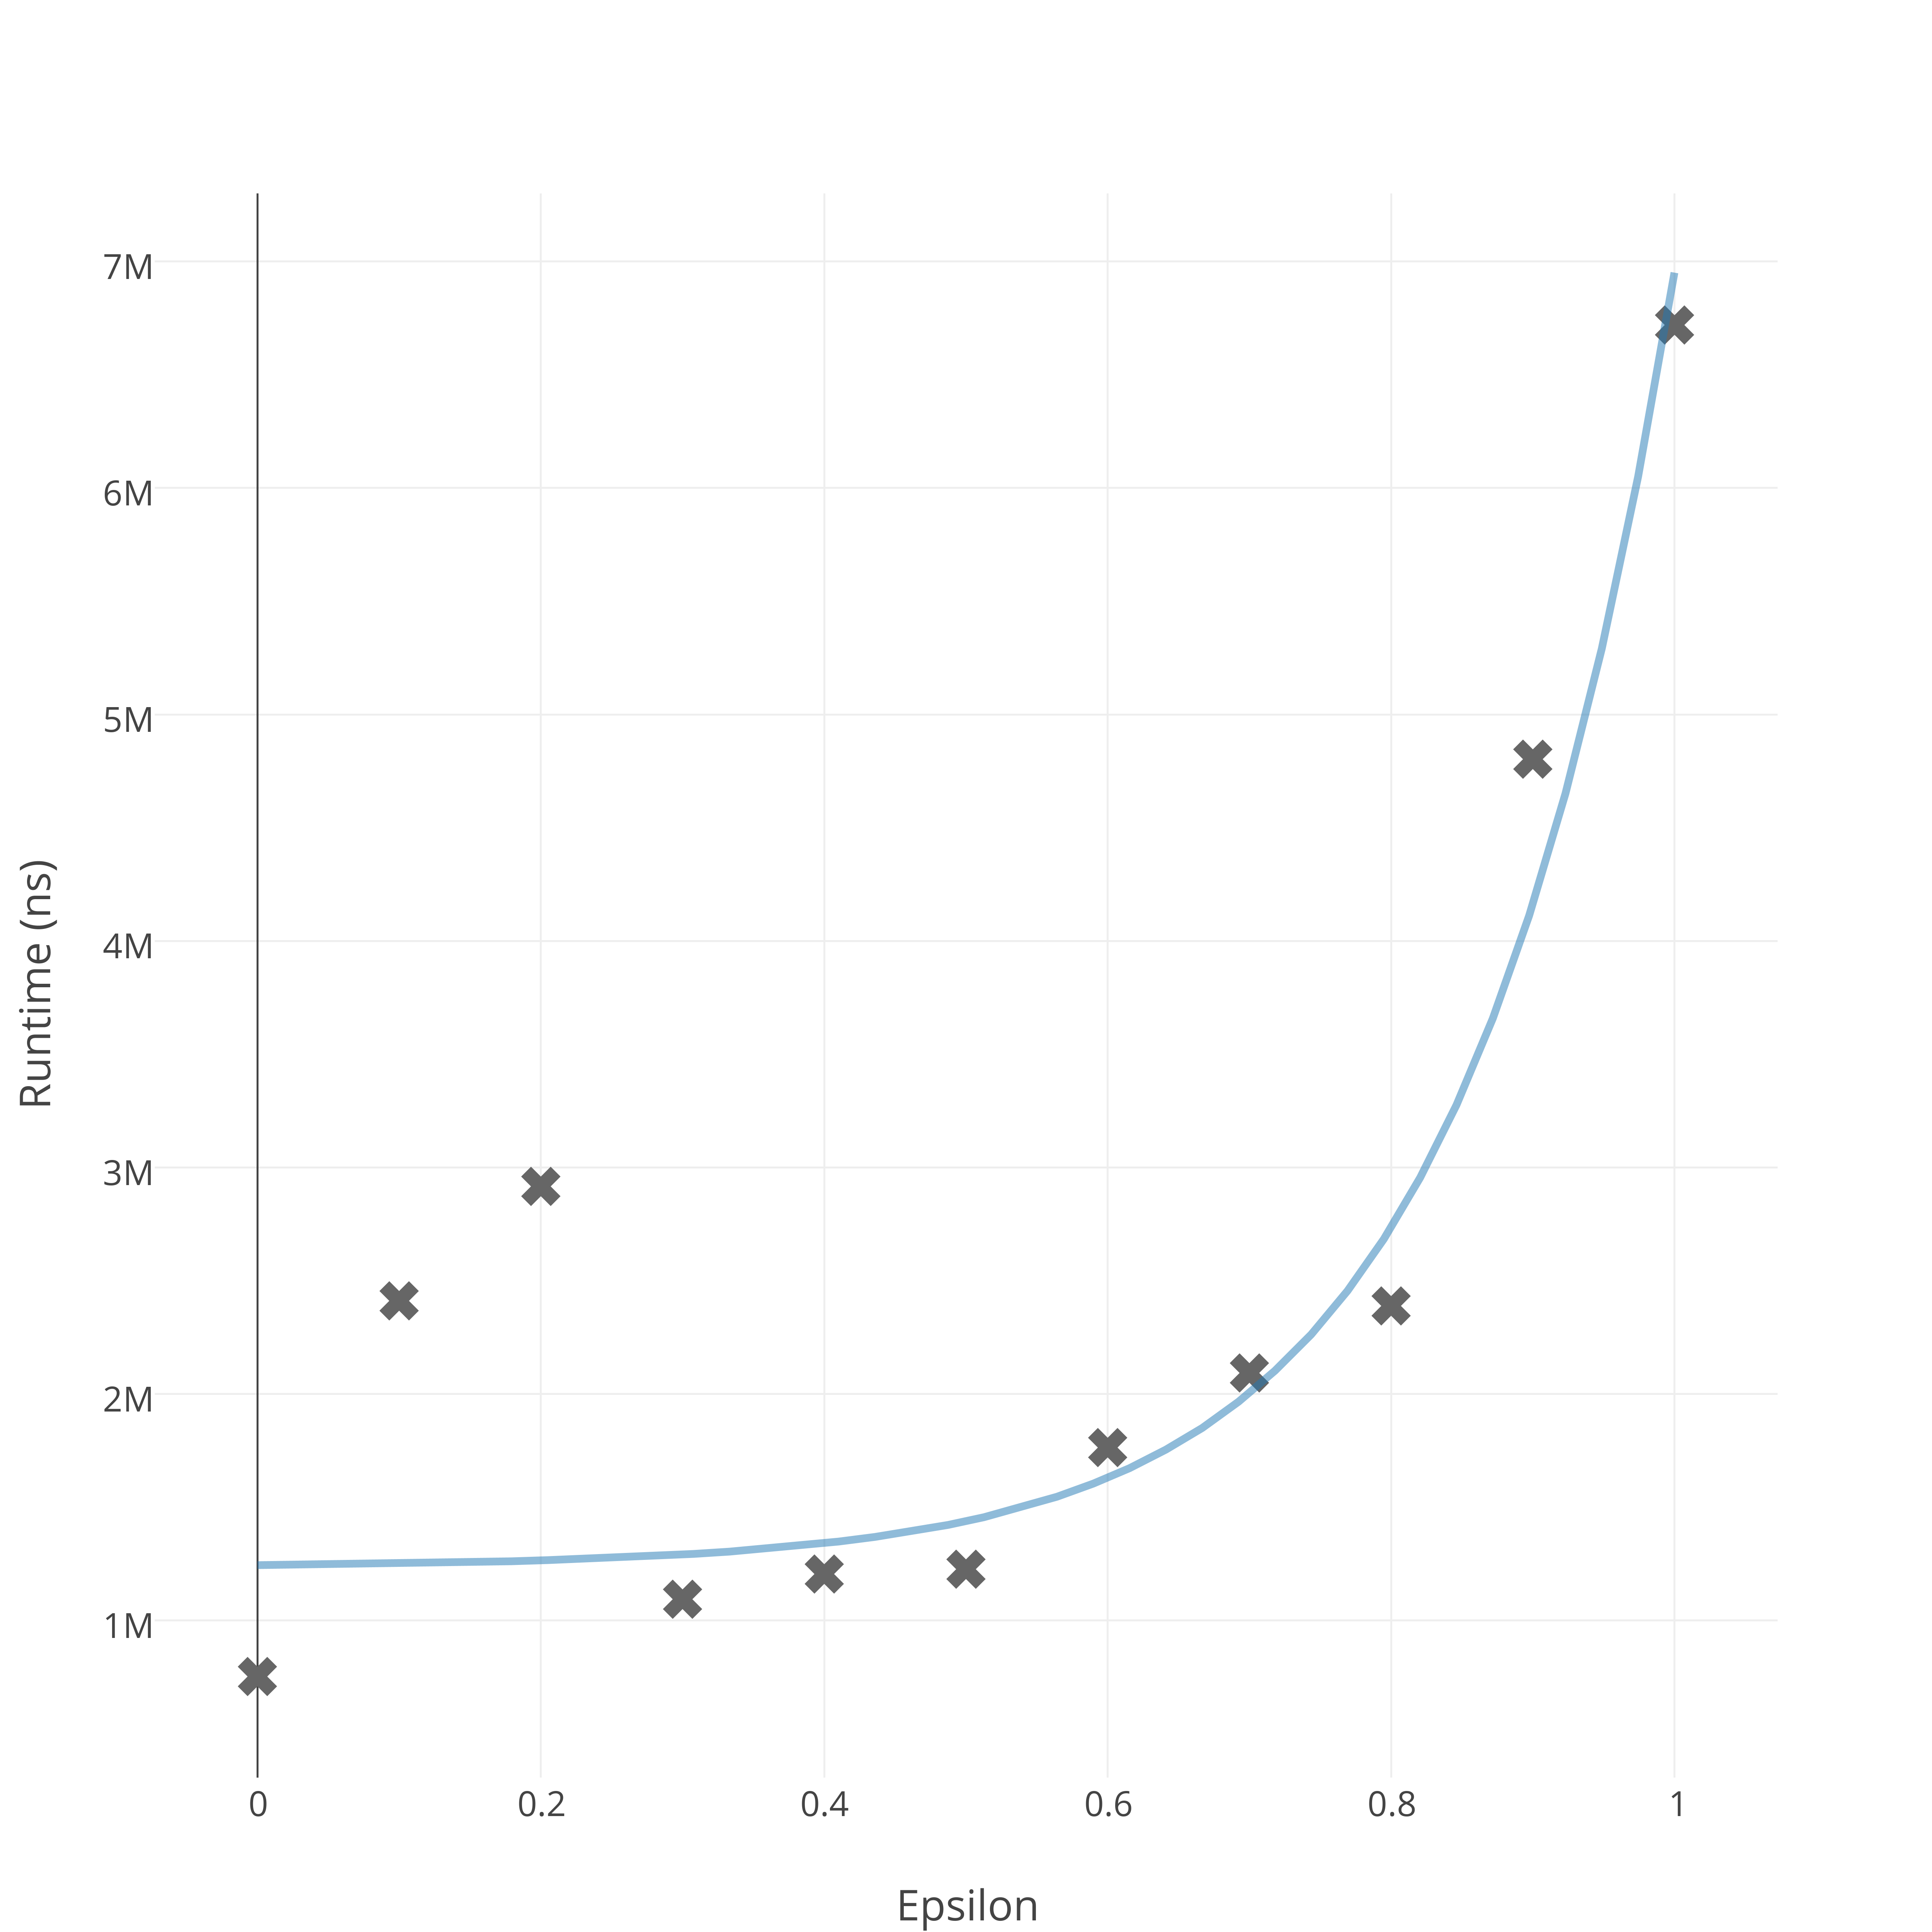
\includegraphics[width=.5\textwidth]{pics/runtimevsepsilon_medium}}{\centering\caption{$\epsilon$ vs runtime for the medium map for Q-learning. An exponential regression is superimposed on the graph.}\label{fig:qlruntimemedium}}
    \end{floatrow}
\end{figure}

\end{document}